%; whizzy chapter
% -initex iniptex -latex platex -format platex -bibtex jbibtex -fmt fmt
% 以上 whizzytex を使用する場合の設定。

%     Tokyo Debian Meeting resources
%     Copyright (C) 2010 Junichi Uekaw
%     Copyright (C) 2010 Nobuhiro Iwamatsu

%     This program is free software; you can redistribute it and/or modify
%     it under the terms of the GNU General Public License as published by
%     the Free Software Foundation; either version 2 of the License, or
%     (at your option) any later version.

%     This program is distributed in the hope that it will be useful,
%     but WITHOUT ANY WARRANTY; without even the implied warranty of
%     MERCHANTABILITY or FITNESS FOR A PARTICULAR PURPOSE.  See the
%     GNU General Public License for more details.

%     You should have received a copy of the GNU General Public License
%     along with this program; if not, write to the Free Software
%     Foundation, Inc., 51 Franklin St, Fifth Floor, Boston, MA  02110-1301 USA

%  preview (shell-command (concat "evince " (replace-regexp-in-string "tex$" "pdf"(buffer-file-name)) "&"))
% 画像ファイルを処理するためにはebbを利用してboundingboxを作成。
%(shell-command "cd image201002; ebb *.png")

%%ここからヘッダ開始。

\documentclass[mingoth,a4paper]{jsarticle}
\usepackage{monthlyreport}

% 日付を定義する、毎月変わります。
\newcommand{\debmtgyear}{2010}
\newcommand{\debmtgmonth}{4}
\newcommand{\debmtgdate}{17}
\newcommand{\debmtgnumber}{63}

\begin{document}

\begin{titlepage}
\thispagestyle{empty}

% タイトルページ:編集必要な部分は最初のマクロに飛ばすこと

\vspace*{-2cm}
第\debmtgnumber{}回 東京エリア Debian 勉強会資料\\
\hspace*{-2cm}
\includegraphics[width=210mm]{image201004/2010title.eps}\\
\hfill{}\debmtgyear{}年\debmtgmonth{}月\debmtgdate{}日

\rotatebox{5}{\fontsize{24}{24} {\gt 特集1: piupartsの使い方}}

\rotatebox{5}{\fontsize{24}{24} {\gt 特集2: debtags入門} }

\vspace*{-2cm}
\end{titlepage}


\begin{minipage}[b]{0.2\hsize}
 \definecolor{titleback}{gray}{0.9}
 \colorbox{titleback}{\rotatebox{90}{\fontsize{80}{80} {\gt デビアン勉強会} }}
\end{minipage}
\begin{minipage}[b]{0.8\hsize}
\hrule
\vspace{2mm}
\hrule
\begin{multicols}{2}
\tableofcontents
\end{multicols}
\vspace{2mm}
\hrule
\end{minipage}

\dancersection{Introduction}{上川 純一}
 
 今月のDebian勉強会へようこそ。これからDebianの世界にあしを踏み入れると
 いう方も、すでにどっぷりとつかっているという方も、月に一回Debianについ
 て語りませんか?

 Debian勉強会の目的は下記です。

 \begin{itemize}
 \item \underline{Debian Developer} (開発者)の育成。
 \item 日本語での「\underline{開発に関する情報}」を整理してまとめ、アップデートする。
 \item \underline{場}の提供。
 \begin{itemize}
  \item 普段ばらばらな場所にいる人々が face-to-face で出会える場を提供
	する。
  \item Debian のためになることを語る場を提供する。
  \item Debianについて語る場を提供する。
 \end{itemize}
 \end{itemize}		

 Debianの勉強会ということで究極的には参加者全員がDebian Packageをがりがり
 と作るスーパーハッカーになった姿を妄想しています。情報の共有・活用を通し
 て Debianの今後の能動的な展開への土台として、「場」としての空間を提供す
 るのが目的です。

\newpage
\dancersection{事前課題}{岩松 信洋}

今回の事前課題は以下です:

\begin{enumerate}
 \item あなたの使っているinitは何ですか?使っている理由を教えてください。
 \item あなたのパッケージ検索方法を教えてください。

\end{enumerate}

この課題に対して提出いただいた内容は以下です。



\begin{prework}{ $B868}=(9/(B }

\begin{enumerate}
\item $B%G%U%)%k%H$N(B2$B$r;HMQ$7$F$$$^$9!#(B
$BDL>o$N%$%s%9%H!<%k$r$7$F$=$N$^$^;HMQ$7$F$$$k$+$i$G$9!#(B
2-5$BA4$FF1$8$J$N$KB>$N%i%s%l%Y%k$r;HMQ$9$k0UL#$O$o$+$C$F$$$^$;$s(B

\item apt-get apptitude$B!"!V%Q%C%1!<%8$NFbMF$r8!:w!W$r;HMQ$7$^$9!#(B
$BL@3N$KL>A0$,J,$+$k$b$N$O(Bapt-get$B$d(Bapptitude$B$G(B
$B$3$&$$$&$b$N$,$[$7$$$H;W$&$H$-$O!V%Q%C%1!<%8$NFbMF$r8!:w!W$r;H$$$^$9!#(B
$B%-!<%o!<%I$,;H$o$l$F$$$J$$%Q%C%1!<%8$G$b8!:w$9$k$3$H$,2DG=$@$+$i$G$9(B
\end{enumerate}

\end{prework}



\begin{prework}{ $B%-%?%O%i(B }
\begin{enumerate}

\item $B%G%U%)%k%H$GAH$_9~$^$l$k!V(Binit$B!W!"FC$KITET9g$,$J$$$?$a!#(B
\item $B:G6a$O!"!V(BGoogle$B@h@8!W$K?R$M$k;v$N$[$&$,B?$$!#(B

\end{enumerate}

\end{prework}



\begin{prework}{ yama1066 }
\begin{enumerate}

\item sysvinit
$B$^$@0\9T$7$F$J$$$+$i!#(B
upstart $B$K0\9T$9$k%a%j%C%H$,5DO@$G$-$l$P$$$$$J$H;W$$$^$9!#(B
\item dselect $B$G$R$?$9$i%4%j%4%j!D!"13$G$9!#(Bapt-cache search $B$G$[$2$[$2!#(B
\end{enumerate}

\end{prework}

\begin{prework}{ henrich }
\begin{enumerate}
\item sysvinit $B$r;H$C$F$^$9!#@N$O(B initng $B$r;H$C$?$3$H$b$"$j$^$7$?$,!D(B
$BLLE]$rHr$1$k$?$a!"$G$9$+$M!#(B
\end{enumerate}

\end{prework}



\begin{prework}{ koedoyoshida }

\begin{enumerate}
\item $B0BDj;V8~$J$N$G(Blenny$BI8=`$N(Binit$B$G$9!#(B
$B;E;v$G;H$C$F$k%^%7%s$O(Bupstart$B$d(Binit$B$,:.:_$7$F$$$^$9!#(B

$B;d$O4pK\E*$K(BLinux$B$O%5!<%P;HMQ$G$9!#(B
$BLGB?$K:F5/F0$7$J$$$N$G$"$^$j287C$r<u$1$F$$$^$;$s!#(B

$BFC$K%a!<%+!<7O$N%5!<%P5!$O(B($B:F(B)$B5/F0;~$K(BSAS,FC$BEy$r4^$a$?(BBIOS$B%A%'%C%/$@$1$G?tJ,$+$+$k$N$b$6$i$J$N$G!"5/F09bB.2=$N%a%j%C%H$O<u$1$K$/$$$H$$$&$N$,@5D>$J$H$3$m$G$9!#(B

init$B0J30$r;HMQ$9$k$3$H$K$h$k!"5/F0;~0J30$N%a%j%C%H$,M-$l$PCN$j$?$$$G$9!#(B

\end{enumerate}

\end{prework}



\begin{prework}{ $BNkLZ?rJ8(B }
\begin{enumerate}
\item sysvinit$B!#(B
$BFC$K%9%T!<%I$r5a$a$h$&$H;W$C$?$3$H$,$J$$$3$H$H!"%5!<%S%95/F0$,HsF14|$@$H2?$+LdBj$,5/$-$?$H$-$KD4::$7$K$/$$%$%a!<%8$,$"$k$?$a!#(B
$B$H$O$$$(!"(BUbuntu$B$N%^%7%s$G$O(BUpstart$B;H$C$F$$$k$N$G!"$?$@N.$5$l$F$$$k$@$1$@$H;W$$$^$9!#(B
\end{enumerate}

\end{prework}



\begin{prework}{ $BF#BtM}Ao(B(risou) }
\begin{enumerate}
\item $B:#;HMQ$7$F$$$k$N$O(B sysvinit $B$G$9!#M}M3$O!"(B lenny $B$N%G%U%)%k%H$K$J$C$F$$$k$+$i$G$9!D!D!#(B
$B!t$3$N$"$?$j!"0c$$$,$h$/$o$+$C$F$J$$$N$G!"$o$6$o$6JQ99$7$F$J$$$G$9!#(B
\end{enumerate}

\end{prework}



\begin{prework}{ $BB<ED?.?M(B }

\begin{enumerate}
\item sysvinit$B!#>/$7A0$K(BSqueeze$B$r%$%s%9%H!<%k$7$?$i%G%U%)%k%H$@$C$?$+$i!#(B
\item  apt-cache search$B$G$6$C$/$j$H8+Ev$r$D$1$F$+$i(Bapt-cache show$B$G>\:Y$r3NG'!#(B
\end{enumerate}
\end{prework}

\begin{prework}{ akedon }

\begin{enumerate}
\item sysvinit $B$G$9!#8=:_!"%G%U%)%k%H$J$N$H%a%+%K%:%`$,C1=c$J$N$G$3$l$GNI$$$+$J$H;W$C$F$$$^$9!#(B
\item aptitude search $B!A(B $B$H(B apt-file search $B!A(B $B$r;H$C$F$$$^$9!#(B
\end{enumerate}
\end{prework}

\begin{prework}{ Hirotaka Kawata }

\begin{enumerate}
\item init$B!#(BDebian $BI8=`$N(B init ($B$U$D$&$N(B init)
\item aptitude search "keyword"
\end{enumerate}
\end{prework}

\begin{prework}{ opentaka }

\begin{enumerate}
\item $B%G%U%)%k%H$N(Binit$B!#%G%U%)%k%H$GF~$C$F$$$?$N$G!#(B
\item aptitude search "package name"
\end{enumerate}
\end{prework}

\begin{prework}{ $B>>_7FsO:(B }
\begin{enumerate}
\item $B$"$^$j0U<1$7$F$$$^$;$s$G$7$?$,!"%G%U%)%k%H$N$b$N$r;H$C$F$$$^$9!#(Bsysvinit?
\item aptitude search hoge
\end{enumerate}
\end{prework}

\begin{prework}{ $B$^$($@$3$&$X$$(B }

\begin{enumerate}
\item sysvinit$B!#%F%9%H4D6-$H$+$G$O(Bupstart$B$b;n$7$F$^$9$,!"(BMacBook$B$N(BSid$B4D6-$H$+$G$O@Z$jBX$($k$N$^$@I]$$$G$9$M!#(B
\item apt-cache
\end{enumerate}
\end{prework}

\begin{prework}{ Yasunori Higashiyama }

\begin{enumerate}
\item sysvinit$B!#FC$K:$$C$F$$$J$$$N$G$=$N$^$^!#(B
\item web$B$G8!:w$+(Baptitude search
\end{enumerate}
\end{prework}

\begin{prework}{ $B4d>>(B $B?.MN(B }

\begin{enumerate}
\item sysvinit $B$G$9!#(BDebian$B$N%G%U%)%k%H$@$+$i$G$9!#(B
\item aptitude $B$G8!:w$7$F$$$^$9(B $B!#%?%0$r;H$$$^$9!#%Q%C%1!<%8$N%$%s%9%H!<(B
      $B%k$O(Bapt $B$G$9$,(B....$B!#$"$H$O!"(Biceweasel$B$d(BGoogle Chrome$B$N8!:w%\%C%/%9$G8!:w$9$k$3$H(B
      $B$b$"$j$^$9!#(B
\end{enumerate}
\end{prework}


\begin{prework}{ google-account@rolf.leggewie.biz }

$B:#2s$b$h$m$7$/$*4j$$$7$^$9!#(B

\end{prework}




\dancersection{最近のDebian関連のミーティング報告}{前田耕平}
\subsection{東京エリアDebian勉強会62回目報告}
% (query-replace-regexp "<.*?>" "")
% (query-replace-regexp "^[	 ]\+" "")

2010年3月の東京エリアDebian勉強会、
参加者は山本さん、日比野さん、岩松信洋さん、吉野与志仁さん、
本庄さん、henrich さん、あけどさん、前田耕平さん、荒木(靖)さん、
吉田@小江戸さん、中尾さん、上川の12人でした。

本庄さんがニューラルネットワークを使って書籍スキャンを便利にしてみた話。
次回はlibsvmとlibsaneを使っていろいろ拡張するそうです。

前田さんが weka を使ってみて、今月の生活費を予測した内容でした。
回帰分析の結果とか、おもしろすぎです。

上川がlibfftw と libsndfile を使ってみた話をしました。

日比野さんが、日本語 man がうまく表示されない件について発表してくれました。
groffの深みについて語り合う会です。
dvi サポートとかを考えるとめんどくさすぎですが、どうしたものか。

吉野さんが、dpkg の新しいソースファイル形式、
3.0 quilt について紹介してくれました。

宴会は銀座ライオン。

\dancersection{Debian Trivia Quiz}{岩松 信洋}

ところで、みなさん Debian 関連の話題においついていますか?Debian関連の話
題はメーリングリストをよんでいると追跡できます。ただよんでいるだけではは
りあいがないので、理解度のテストをします。特に一人だけでは意味がわからな
いところもあるかも知れません。みんなで一緒に読んでみましょう。

今回の出題範囲は\url{debian-devel-announce@lists.debian.org} に投稿された
内容とDebian Project Newsからです。

\begin{multicols}{2}
 %; whizzy-master ../debianmeetingresume200906.tex
% $B0J>e$N@_Dj$r$7$F$$$k$?$a!"$3$N%U%!%$%k$G(B M-x whizzytex $B$9$k$H!"(Bwhizzytex$B$,MxMQ$G$-$^$9!#(B
%
% $B$A$J$_$K!"%/%$%:$OJL%V%i%s%A$G:n@.$7!"$N$A$K%^!<%8$7$^$9!#5U$K%^!<%8$7(B
% $B$J$$$h$&$K$7$^$7$g$&!#(B
% (shell-command "git checkout quiz-prepare")

\santaku
{DPL 2010 $B$KN)8uJd$7$F$$$k$N$OC/!)(B}
{Yasuhiro Araki} % JP 
{Charles Plessy}
{Kurt Roeckx}
{B}

\santaku
{Debian policy 3.8.4.0$B$GDI2C$5$l$?9`L\$O!)(B}
{/sys $B$H(B /selinux $B$N(BFHS$B$KBP$9$kNc30%]%j%7!<(B}
{kFreeBSD$B$H(BLinux$B$r6&B8$9$k%]%j%7!<(B}
{$B%9!<%Q5m$5$s%Q%o!<$K4X$9$k%]%j%7!<(B}
{A}

\santaku
{$B:G6a%O!<%I%&%'%"%H%i%V%k$,$"$C$?%5!<%P$O!)(B}
{rie.debian.org}
{ries.debian.org} % ftp-master.debian.org
{rise.debian.org }
{B}

\santaku
{buildd.debian.org$B$N$"$k%5!<%P$,0\F0$7$^$7$?!#$I$3$K0\F0$7$?$G$7$g$&!#(B}
{peri.debian.org} % ppc buildd
{cimarosa.debian.org} % $B0\F0A0(B
{grieg.debian.org} % $B0\F08e(B
{C}

\santaku
{squeeze$B$N%$%s%9%H!<%i$GDI2C$5$l$?5!G=$O(B}
{Recommends$B$r%$%s%9%H!<%k$9$k$h$&$K$7$^$9(B}
{$B%$%s%9%H!<%i>e$G%Q%C%1!<%8$,%S%k%I$G$-$^$9(B}
{$B%/%m%9%"!<%-%F%/%A%c%$%s%9%H!<%k5!G=$rDI2C$7$^$7$?(B}
{A}

\santaku
{$B?7$7$/(Bmips$BMQ(Bporterbox$B$,DI2C$5$l$^$7$?!#(BCPU$B%3%"?t$O$$$/$D$G$7$g$&$+!#(B}
{64}
{32}
{16}
{C}

\end{multicols}

\clearpage

%\dancersection{libsane 入門}{本庄}
%\dancersection{debhelper v7 でのパッケージ管理}{誰か}
%\dancersection{死屍累々のundefoma 、その後は?}{誰か}
\dancersection{piuparts の使い方}{岩松}

\subsection{はじめに}
piuparts は 次期リリース squeeze の目標の一つに挙げられている
\texttt{Package clean install/uninstall}を達成するためのサポートツールです。
既に構築されたDebianパッケージのインストール、アンインストール、アップグ
レードのチェックを行います。
通常、パッケージ構築時の依存関係チェックや実際の構築には\texttt{pbuilder/cowbuilder}を使
います。パッケージのインストール、動作確認までは行いますが、アンインストー
ルまでの確認を行っているパッケージメンテナは少ないようで(実際にそのまま
使う人が多いためと考えられる)、アンインストールできない事が稀にありまし
た。最悪の場合、パッケージを作ってテストせずにアップーロードしてしまう事
もあるようです。また、stable からのアップグレードチェックもパッケージメ
ンテナはあまりやってないのではないでしょうか。
このような問題をチェックするためのツールとして\texttt{piuparts}は作られました。
では、\texttt{piuparts}はどのように動き、どのように使うのか見ていきましょう。

\subsection{piupartsの使い方}

\texttt{piuparts}を使ってパッケージのチェックを行う場合には、
\texttt{piuparts}コマンドにチェックしたいパッケージを指定します。
例えば、\texttt{libcv4\_2.0.0-4\_i386.deb}パッケージをチェックしてその結果
を\texttt{/tmp/libcv4\_2.0.0-4\_i386.piuparts-log}に保存する場合には以
下のように実行します。
実行するとログが標準出力にも出力されますが、\texttt{-l}オプションで指定
したログ指定先にも保存されます。
出力されるログからパッケージのインストール、アンインストール、アップグレードを確認
することができます。

\begin{commandline}
$ sudo piuparts libcv4_2.0.0-4_i386.deb -l /tmp/libcv4_2.0.0-4_i386.piuparts-log
0m0.0s INFO: ------------------------------------------------------------------------------
0m0.0s INFO: To quickly glance what went wrong, scroll down to the bottom of this logfile.
0m0.0s INFO: FAQ available at http://wiki.debian.org/piuparts/FAQ
0m0.0s INFO: ------------------------------------------------------------------------------
0m0.0s INFO: piuparts version 0.38 starting up.
0m0.0s INFO: Command line arguments: /usr/sbin/piuparts libcv4_2.0.0-4_i386.deb -l /tmp/libcv4_2.0.0-4_i386.piuparts-log
0m0.0s INFO: Running on: Linux chimagu 2.6.31-1-686 #1
 SMP Sun Nov 15 20:39:33 UTC 2009 i686
0m0.0s DEBUG: Starting command: ['dpkg', '--info', 'libcv4_2.0.0-4_i386.deb']
0m0.2s DUMP:
.... 省略 .....
6m32.6s DEBUG: Starting command: ['chroot',
 '/tmp/tmplunhrZ', 'umount', '/proc']
6m32.6s DEBUG: Command ok: ['chroot',
 '/tmp/tmplunhrZ', 'umount', '/proc']
6m33.0s DEBUG: Removed directory tree at /tmp/tmplunhrZ
6m33.0s INFO: PASS: All tests.
6m33.0s INFO: piuparts run ends.
\end{commandline}

\texttt{piuparts}の使い方は大きくわけて2つあります。一つはローカルPCにあるパッケージをチェッ
クする場合、もう一つは既にDebianにインストールされているパッケージをチェックす
る場合に使います。
前者はパッケージメンテナがよく使う方法です。パッケージをアップロードする
前にパッケージを指定してテストします。
後者の場合はあまりメンテナはあまり使う機会はないと思いますが、後で説明す
る\texttt{piuparts.debian.org}で使われています。

\subsection{piupartsの動作}
では、\texttt{piuparts}の動作を見てみましょう。状態遷移図を図\ref{fig:piuparts-process}に示します。
非常にシンプルなチェック方法になっていることがわかります。

\begin{figure}[H]
\caption{piupartsの動作}
\begin{center}
\includegraphics[height=0.8\hsize]{image201004/piuparts-process.eps}
\label{fig:piuparts-process}
\end{center}
\end{figure}

大まかな動きは以上になりますが、内部ではdpkg、aptの動きを利用したものに
なっています。
例えば、パッケージのインストールチェックは以下のような動きになっています。
\begin{enumerate}
\item \texttt{dpkg -i} で 指定されたパッケージをインストールする。\\
依存するパッケージがあるばあい、これは失敗する。
\item \texttt{apt-get -yf --no-remove} でパッケージの依存関係をaptで回避してイン
      ストールする。
\end{enumerate}
これは、パッケージ依存関係をパッケージ情報から抽出して指定する方法を取ら
ず、aptのチェック機構を用いて依存関係を回避しようとしています。

\subsection{ログの見方}
\texttt{piuparts}はログが多いので正しい動きをしているのか非常にわかりずらいです。
どのように見たらよいのか簡単に説明します。

\texttt{piuparts}のログは、基本的に以下の順で出力されます。
\begin{enumerate}
\item コマンド実行({\bf DEBUG: Starting command:})
\item 実行開始タグ({\bf DUMP:})
\item 実行時のログ
\item コマンド結果({\bf ERROR:} or {\bf DEBUG: Command ok})
\end{enumerate}
そして、最後にテスト結果が出力されます。
次にテストが正常に終了した場合と、問題がある場合を見てみます。

\subsubsection{テストが正常に終了した場合}

テストに問題がない場合には、以下のように出力されます。
インストール $\rightarrow$ アンインストール、インストール $\rightarrow$ アッ
プグレード $\rightarrow$ アンインストール のチェックが正常に終了しているこ
とがわかります。
\begin{commandline}
.....省略.....
6m13.7s INFO: PASS: Installation and purging test.
.....省略.....
6m32.6s INFO: PASS: Installation, upgrade and purging tests.
.....省略.....
6m33.0s INFO: PASS: All tests.
6m33.0s INFO: piuparts run ends.
\end{commandline}

\subsubsection{エラーがある場合}

エラーがある場合には、{\bf ERROR:}の次にエラー内容がされます。
以下に、実際のエラー内容を示します。
これは、upstartのチェック結果ですが、essentialパッケージである、sysvinit
をアンインストールしようとして、エラーになっています。

\begin{commandline}
0m6.0s DEBUG: Starting command: ['chroot', '/org/piuparts.debian.org/tmp/tmpZ-SX9D', 'apt-get', '-y', 'install', 'upstart']
^^^^^^^^^^^^^^^^^^^^^^^^^^^^^^: コマンド実行
0m6.3s DUMP:
^^^^^^^^^^^: コマンド実行時の情報
  Reading package lists...
  Building dependency tree...
  The following extra packages will be installed:
    libdbus-1-3
  Recommended packages:
    dbus
  The following packages will be REMOVED:
    sysvinit
  The following NEW packages will be installed:
    libdbus-1-3 upstart
  WARNING: The following essential packages will be removed.
  This should NOT be done unless you know exactly what you are doing!
    sysvinit
  0 upgraded, 2 newly installed, 1 to remove and 0 not upgraded.
  Need to get 636kB of archives.
  After this operation, 1196kB of additional disk space will be used.
  E: There are problems and -y was used without --force-yes
0m6.3s ERROR: Command failed (status=100): ['chroot', '/org/piuparts.debian.org/tmp/tmpZ-SX9D', 'apt-get', '-y', 'install', 'upstart']
^^^^^^^^^^^^: コマンド結果
\end{commandline}

\subsection{piupartsのオプション}
普通の使い方では使いづらいので、\texttt{piuparts}で提供されているオプションを
自分が使っている開発環境に合わせて使うのが普通のようです。以下では
よく使うオプションを紹介します。

\subsubsection{pbuilderのbase.tgzをpiupartsで利用する}
\texttt{piuparts}はテストする度にbaseイメージを構成するパッケージ群をミラーサーバ
から取得し、baseイメージを構築します。キャッシュする機構はいまのところ存
在せず、毎回取得する仕様になっています。これではサーバに負荷がかかります。
そこで、\texttt{-p}オプションを使います。 このオプションはpbuilderのbaseイメー
ジ\texttt{/var/cache/pbuilder/base.tgz}を使ってテストを行うオプションで
す。
通常、パッケージメンテナは pbuilder/cowbuilderを使ってパッケージビルドチェック
を行うので、便利なオプションの一つです。
また、pbuilderを使ってないが、base.tgzを独自のスクリプトで保持している人
もいるでしょう。この場合には\texttt{--basetgz}オプションでtgzファイルを
指定することによって、利用できます。

\subsubsection{ディストリビューションの指定}
piupartsは unstable(sid)だけでなく、現在サポートされているDebianのディストリビュー
ションとUbuntuのディストリビューションをサポートしています。
ディストリビューションの指定には\texttt{-d}オプションを指定します。
これは複数指定することができ、指定した順にテストが実行されます。
以下の例では、sid環境を構築し、テストした後、squeeze の環境を構築し、テ
ストします。
\begin{commandline}
$ sudo piuparts -d sid -d squeeze libcv4_2.0.0-4_i386.deb
.....
\end{commandline}

\subsection{debianにインストールされているパッケージのテスト}
既に debian にインストールされているパッケージのテストを行う場合には、
\texttt{--apt}オプションを使います。
特定のディストリビューションにあるパッケージのテストを行いたい場合には、
\texttt{-d}オプションでディストリビューションを指定する必要があります。

\begin{commandline}
$ sudo piuparts --apt -d squeeze libcv4
\end{commandline}

\subsubsection{ミラーサーバの指定}
デフォルトでは、\texttt{piuparts}が使うDebianリポジトリは、
\texttt{/etc/apt/sources.list}からパーサして利用します。
一家に一台Debianミラーの時代です。グローバルなミラーサーバを使用せず
にローカルにあるミラーサーバを指定する場合には、\texttt{--mirror}オプショ
ンを使って指定します。

\begin{commandline}
$ sudo piuparts -p libcv4_2.0.0-4_i386.deb --mirror http://debmirror.example.org/debian
\end{commandline}

\subsubsection{依存するパッケージの回避方法}
通常、ライブラリソースパッケージはlibfoo0、libfoo-dev など複数のバイナリパッケージを生
成します。この場合、libfoo-dev パッケージは libfoo0 パッケージに依存して
いるので、libfoo-devパッケージだけでテストしても、libfoo0がないのでテス
トでエラーになります。
この場合には、パッケージを2つ(libfoo0, libfoo-dev)指定することで回避でき
ます。

\begin{commandline}
$ sudo piuparts -p libcv-dev_2.0.0-4_i386.deb libcv4_2.0.0-4_i386.deb
\end{commandline}

また、ソースパッケージから作成されたバイナリパッケージのテストを行う場合
には、\texttt{*.changes}ファイルを指定します。

\begin{commandline}
$ sudo piuparts -p opencv_2.0.0-4_i386.changes
\end{commandline}

\subsection{piuparts.debian.org}
piupartsがパッケージとして用意されたとしても、まだ利用しているパッケージ
メンテナは少ないようです。また、パッケージ作成時には問題がなかったが、依
存関係があるパッケージが更新および削除され、正常にインストール等ができな
い状態になる場合があります。
そこで、QAチームは既にDebianにインストールされ
たパッケージをチェックするためのサービス\texttt{piuparts.debian.org}を立
ち上げました。
これでチェックされた内容は、\texttt{qa.debian.org}で提供されている情報の
一部として、表示されています。

\subsubsection{現在チェックエラーになっているパッケージ}

\texttt{piuparts}でチェックでエラーになっているパッケージはタグとユーザダグで検索できます。
\begin{itemize}
\item タグ : piuparts
\item ユーザタグ : debian-qa@lists.debian.org
\end{itemize}

BTSでは以下のURLで参照できます。
\url{http://bugs.debian.org/cgi-bin/pkgreport.cgi?tag=piuparts;users=debian-qa@lists.debian.org}

\subsection{現在の問題点}
現在、piupartsにはいくつかの問題点があります。
\url{http://packages.qa.debian.org}で表示されるチェック結果が誤解を受け
やすいという点です。
依存しているパッケージが問題を持っているのに、それが自分のパッケージにエラーとなって
表示されます。情報を追えばどのパッケージでエラーになっているのか分かりま
すが、情報を追うのがめんどうです。

細かいところでは、\texttt{-B}の使い方がわかりません。
\begin{commandline}
$ piuparts --help
.... 中略 ....
 -B FILE, --end-meta=FILE
                     XXX
\end{commandline}
ちなみに \#560050で 報告されていますが、開発者本人が報告しているので修正する
気がないのかもしれません。

\subsection{まとめ}

今回は基本的な使い方と、パッケージメンテナから利用する場合に使うオプショ
ンを説明しました。パッケージメンテナの方は自分でもっているパッケージテス
トに組み込んでみてはいかがでしょうか。パッケージの基本的な部分の問題が
減るのでよいと思います。

また、現在piuparts v2 を開発中です。開発はbzr上で行われています。
\url{http://code.liw.fi/piuparts2/bzr/trunk/}
ソースコードも多くなく、やっていることも単純です。
興味のある方は参加してみてはいかがでしょうか。

\dancersection{upstart 再入門}{前田耕平}

\subsection{はじめに}
今年の2月の Debian 勉強会(Debian 温泉)で一度扱ったテーマですが、新年度
も始まり、新入生、新入社員、新入 Debian 開発者予備軍の皆さんも、気分も新
たに、いずれやってくるであろう、Squeeze のリリースに備えもう一度おさらい
しておきましょう。
\footnote{書き下ろすつもりでしたが、個人的な都合で余裕がなく、今回の事前配布資料は基本的に、2010年2月の Debian 勉強会の資料「ブート方法が変
わるよ」を再編したものです。}

\subsection{従来のinit}

まず従来の init のおさらいです。従来の init はSystem V 系の Unix 由来の
起動の仕組みで、sysvinit といい、 Unix/Linux システムにおいて、カーネル
がブートした後、ユーザプログラムが起動するための仕組みです。マシンに電源
を入れてからログインプロンプトが表示されるまの流れは大まかには次のように
なります。

\begin{figure}[H]
\caption{ブートの流れ}
\begin{center}
\includegraphics[height=0.5\hsize]{image201002/sysvinit.eps}
\end{center}
\end{figure}

init プロセスが起動すると、init は /etc/inittab の内容に従って、プロセス
のを生成や停止を行います。inittab の書式は次のとおりです。

\begin{commandline}
id:runlevels:action:process
\end{commandline}

Debian システムのデフォルトランレベルは 2 なので、プロセスの生成に関わる
基本的なエントリは次の4行です。

\begin{commandline}
id:2:initdefault:                     ←デフォルトランレベルは2
si::sysinit:/etc/init.d/rcS           ←起動時は必ず実行
l2:2:wait:/etc/init.d/rc 2            ←ランレベル 2で実行。
1:2345:respawn:/sbin/getty 38400 tty1 ← getty を常駐
\end{commandline}

2行目のエントリは、ランレベルが指定されてませんが、action に sysinit が指定されているた
めです。これはシステムブート中に他のブート用の action よりも優先して実行
されます。ここで実行される /etc/init.d/rcS では

\begin{commandline}
exec /etc/init.d/rc S
\end{commandline}

とだけが実行されます。これはランレベル S のシングルユーザモードのときのも
のです。上記3行目でランレベル 2のときに実行されるエントリがあることから
も分かるとおり、
\begin{enumerate}
 \item ランレベル Sのプロセスが実行
 \item ランレベル 2のプロセスが実行
\end{enumerate}
の順で起動プロセスが実行されます。ランレベル S 用の起動処理が終わってか
ら、ランレベル 2 用の起動処理が実行されるのですから、/etc/rcS.d/ 以下と
/etc/rc2.d/ 以下を比較しても分かるとおり、これが逐次実行されるのはかなり
時間がかかるでしょう。

\subsection{upstart の特徴}

upstart は sysvinit をイベントベースに置き換えたもので、
サービスの開始と停止はイベントの通信にもとづきます。

upstart の特徴は次の6つです。

\begin{itemize}
 \item イベントドリブンでタスクやサービスを起動・停止する。
 \item タスクやサービスが起動・停止することでイベントが発生する。
 \item イベントはシステム上の他のプロセスから受け取ることができる。
 \item サービスが予期せず突然終了しても再起動することができる。
 \item デーモンの監視と再起動は親プロセスから分離できる。
 \item D-Bus を通じて init デーモンと通信できる。
\end{itemize}

upstart の状態遷移は次の図のようになります。

\begin{figure}[thbp]
\begin{center}
\caption{upstart 状態遷移}
\includegraphics[height=0.7\hsize]{image201002/states.eps}
\end{center}
\end{figure}

\clearpage

upstartは、sysvinitと同様な機能を提供しますが、\textbf{非同期イベントに
応じて自律的に動作する点}がもっとも異なります。そのため、sysvinit に対す
る upstart のメリットには、
\begin{itemize}
 \item 利用可能なハードウェアだけでブートするため、runlevel が必要ない。
       これは存在しないハードウェアを必要とするジョブをトリガーとしない
       ため。
 \item ホットプラグデバイスに対応
\end{itemize}
といったことが挙げられます。

例えば、システムがブート後、NICを挿すと
\begin{enumerate}
 \item network-interface-add イベント生成
 \item DHCPジョブがネットワークカードを構成
 \item network-interface-upイベントが生成
 \item デフォルトルートが新しいインタフェースに割り当て
 \item default-route-upイベントが生成
 \item NICを必要とするジョブ(各種サーバ)が自動的に開始される
\end{enumerate}

逆にネットワークカードがなくなった場合は自動的に停止されます。

\subsubsection{upstartへ の切り替え}

切り替えには upstart パッケージをインストールします。通常のパッケージのインストールとは異なり、続行する場合は、\textbf{Yes, do as I say}と入力しなさい、というメッセージが表示されます。
これはうまくいかない場合は Debian システムが起動できなくなるなどのリスク
があるためです。

\begin{commandline}
$ sudo apt-get install upstart
パッケージリストを読み込んでいます... 完了
依存関係ツリーを作成しています                
状態情報を読み取っています... 完了
以下の特別パッケージがインストールされます:
  dbus libdbus-1-3 libexpat1
提案パッケージ:
  dbus-x11
以下のパッケージは「削除」されます:
  sysvinit
以下のパッケージが新たにインストールされます:
  dbus libdbus-1-3 libexpat1 upstart
警告: 以下の不可欠パッケージが削除されます。
何をしようとしているか本当にわかっていない場合は、実行してはいけません!
  sysvinit
アップグレード: 0 個、新規インストール: 4 個、削除: 1 個、保留: 9 個。
1,005kB のアーカイブを取得する必要があります。
この操作後に追加で 2,105kB のディスク容量が消費されます。
重大な問題を引き起こす可能性のあることをしようとしています。
続行するには、'Yes, do as I say!' というフレーズをタイプしてください。
 ?] Yes, do as I say!
\end{commandline}

2月の Debian 勉強会時点で、lxc の環境で試した際\footnote{2010年2月9日現
在}は、getty がうまく動かず、起動しては突然死して、再起動されて、また突
然死、というのを繰り返してしまい、コンソールからのログインは出来ない状態
でしたが、今回の資料作成時点\footnote{2010年4月11日に、Squeeze Official
Snapshot amd64 BC Binary-1 20100322-03:30の ISO イメージを使用した最小構
成。}では、
KVM環境で問題なく起動します。バージョンが変わってませんが、環境が異なる
ので原因は後者にありそうではあります。

\subsection{参考資料}

\url{http://www.ibm.com/developerworks/jp/linux/library/l-boot-faster/index.html}

%-------------------------------------------------------------------------------
\dancersection{debtags 入門}{やまねひでき}
%-------------------------------------------------------------------------------
\index{debtags}
\subsection{概要}
今日ここでは、「debtags 便利だぜ!」というのと
「もっと便利にするためにオラに元気を分けてくれ!」というのを説明します。

\subsubsection{探し物は何ですか?}
Debian には大量のパッケージが用意されていますが、
最初から全てがインストールされているわけではないので、必要に応じて導入を行います。
で、必要なパッケージがわかっているのならば良いですがそうでない場合も度々です。
その場合にはパッケージの検索を行ってパッケージを見つけてインストールという流れになります。

欲しいファイル・機能を思いつく
→
適当なキーワードで検索
→
見つけたパッケージをインストール

これが多くの Debian ユーザが一般的に行っている流れではないかと思います。

\subsubsection{見つけにくいモノですか?}

通常の apt-cache/aptitude/synaptic の検索 (search オプション) では、
単純なキーワードマッチ検索を行います。
しかし、キーワードにマッチするパッケージが少ない場合はともかく、
大量にマッチしてしまう一般的なキーワードしか思いつかない場合は、
ノイズ混じりの検索結果になって一苦労します。

例えば、ウェブブラウザを普段使っているものから変更したいと思ってパッケージを探してみましょう。

\begin{commandline}
$ apt-cache search web browser| wc -l
295
\end{commandline}

いくら Debian にはパッケージが多いといってもこれは多すぎですね。
その中身をちょっと見てみると…?

\begin{commandline}
<snip>
tor - anonymizing overlay network for TCP
torrentflux - web based, feature-rich BitTorrent download manager
trac-graphviz - Graphs printing plugin for Trac
unhtml - Remove the markup tags from an HTML file
uzbl - Lightweight Webkit browser following the UNIX philosophy
vdetelweb - Telnet and Web interface for VDE 2.x
iceweasel-vimperator - Iceweasel extension to make it have vim look and feel.
<snip>
wwwoffle - World Wide Web OFFline Explorer
xdg-utils - desktop integration utilities from freedesktop.org
xemacs21-bin - highly customizable text editor -- support binaries
xemacs21-gnome-mule-canna-wnn - highly customizable text editor -- transitional package
xemacs21-gnome-mule - highly customizable text editor -- transitional package
xemacs21-gnome-nomule - highly customizable text editor -- transitional package
xemacs21-mule-canna-wnn - highly customizable text editor -- Mule binary compiled with Canna and Wnn
xemacs21-mule - highly customizable text editor -- Mule binary
xemacs21-nomule - highly customizable text editor -- Non-mule binary
xemacs21-support - highly customizable text editor -- architecture independent support files
xemacs21-supportel - highly customizable text editor -- non-required library files
xemacs21 - highly customizable text editor
<snip>
\end{commandline}

ネット接続の匿名化ツールである tor やブラウザのプラグインである iceweasel-vimperator、
さらには xemacs21 のパッケージ群までもが検索一覧に含まれてしまっています。
これは期待している「ウェブブラウザ」の検索結果ではありません。

ではどうすれば効率的にできるのか?そこで debtags ですよ。

\subsection{debtags を導入してつかってみよう}
では早速 debtags を導入してみましょう。
\begin{commandline}
$ sudo aptitude install debtags
\end{commandline}
これだけです。簡単ですね。では実際の検索を。

\begin{commandline}
$ sudo debtags update
$ debtags search web::browser
arora - simple cross platform web browser
chimera2 - Web browser for X
conkeror - keyboard focused web browser with Emacs look and feel
dillo - Small and fast web browser
edbrowse - A /bin/ed-alike webbrowser written in C
elinks - advanced text-mode WWW browser
elinks-lite - advanced text-mode WWW browser - lightweight version
epiphany-browser - Intuitive GNOME web browser
epiphany-extensions - Extensions for Epiphany web browser
epiphany-gecko - Dummy, transitional package
epiphany-webkit - Dummy, transitional package
ezmlm-browse - Web browser for ezmlm-idx archives
galeon - GNOME web browser for advanced users
galeon-common - data for the galeon web browser
iceape-browser - Iceape Navigator (Internet browser) and Composer
iceweasel - Web browser based on Firefox
(snip)
w3m - WWW browsable pager with excellent tables/frames support
w3m-el - simple Emacs interface of w3m
w3m-el-snapshot - simple Emacs interface of w3m (development version)
w3m-img - inline image extension support utilities for w3m
wapua - Web browser for WAP WML pages
\end{commandline}

先ほどよりはずっとまともな情報が検索できるようになっています。
キーワードの組み合わせ方が思いつかないという方も、auto complete があるので安心です。

\begin{commandline}
$ debtags search web(タブキーで補完)
$ debtags search web\:\:(さらにタブキーで補完)
web::TODO           web::browser        web::forum          web::server
web::application    web::cgi            web::portal         web::wiki
web::appserver      web::cms            web::scripting
web::blog           web::commerce       web::search-engine
\end{commandline}

さらに複数のキーワードを組み合わせての検索もお手の物です。
'' でくくって \&\& で組み合わせるだけです。

\begin{commandline}
$ debtags search 'web::browser && x11::application'
arora - simple cross platform web browser
chimera2 - Web browser for X
conkeror - keyboard focused web browser with Emacs look and feel
dillo - Small and fast web browser
epiphany-browser - Intuitive GNOME web browser
epiphany-extensions - Extensions for Epiphany web browser
epiphany-gecko - Dummy, transitional package
epiphany-webkit - Dummy, transitional package
galeon - GNOME web browser for advanced users
galeon-common - data for the galeon web browser
iceape-browser - Iceape Navigator (Internet browser) and Composer
iceweasel - Web browser based on Firefox
junior-internet - Debian Jr. Internet tools
kazehakase - GTK+-based web browser that allows pluggable rendering engines
konq-plugins - plugins for Konqueror, the KDE file/web/doc browser
konqueror - KDE 4's advanced file manager, web browser and document viewer
links2 - Web browser running in both graphics and text mode
midori - fast, lightweight graphical web browser
netsurf-gtk - Small portable web browser with CSS and Unicode support - GTK version
w3m-el-snapshot - simple Emacs interface of w3m (development version)
wapua - Web browser for WAP WML pages
\end{commandline}

これで「X 上のウェブブラウザっていったらどんなのがあるの?」が検索できました。
他に役立ちそうな例としては「ruby の deb パッケージ開発環境を整えたい」などはいかがでしょう?

\begin{commandline}
$ debtags search 'devel::lang:ruby && devel::packaging'
dpkg-ruby - ruby interface for dpkg
ruby-pkg-tools - Tools for building Debian Ruby packages
rubygems1.8 - package management framework for Ruby libraries/applications
\end{commandline}

便利さがいまいちわからない場合は、同じ検索を apt-cache/aptitude のキーワード検索で行ってみてください。
debtags rocks!

ちなみに、
\begin{commandline}
aptitude ~Gdevel::lang:ruby
\end{commandline}
などとして aptitude をインターフェイスとしてタグ検索が可能になっています(ので、そちらが主に使われるようです)。さらについ先日から、新しいインターフェイスとして axi-cache search が使えるようになりました。

\begin{commandline}
$ axi-cache search implemented-in::ruby devel::packaging
182 results found.
Results 1-20:
100% libcairo-ruby1.8 - Cairo bindings for the Ruby language
100% tictactoe - tic-tac-toe game written in Ruby
100% libgnomecanvas2-ruby1.8 - GNOME Canvas 2 bindings for the Ruby language
100% flvtool2 - a manipulation tool for flash video files
100% dpkg-ruby - ruby interface for dpkg
100% libfilesystem-ruby1.8 - Ruby1.8 extension for file-system information
100% libexif-ruby1.9.1 - EXIF tag parsing Library for ruby1.9.1
100% xmms2-scrobbler - Audioscrobbler/Last.FM client for XMMS2
100% ri1.9 - Ruby Interactive reference (for Ruby 1.9)
100% libdbm-ruby - DBM interface for Ruby
100% schleuder - GnuPG enabled mailing list manager with remailer-capabilities
100% libactiveldap-ruby1.8 - an object-oriented interface to LDAP for Ruby
100% libhttp-access2-ruby1.8 - HTTP accessing library for ruby (transitional package)
100% quickml - Very-easy-to-use mailing list system
100% libreadline-ruby1.9.1 - Readline interface for Ruby 1.9.1
100% docdiff - Compares two files word by word / char by char
100% zonecheck-cgi - DNS configuration checker (web interface)
100% libactiveldap-ruby - an object-oriented interface to LDAP for Ruby
100% ohai - Detects data about your operating system and reports it in JSON
100% ditz - distributed issue tracker
More terms: ruby ruby1.8 dependency libactiveldap activeldap interface oriented
More tags: devel::lang:ruby role::program mail::list role::shared-lib devel::library works-with::db interface::commandline
`axi-cache more' will give more results
\end{commandline}

おまけ
\begin{commandline}
$ debtags search 'devel::lang:lisp && devel::packaging'
common-lisp-controller - Common Lisp source and compiler manager
dh-lisp - Debhelper to support Common Lisp related packages
$ 
$ debtags search 'devel::lang:haskell && devel::packaging'
haskell-devscripts - Tools to help Debian developers build Haskell packages
libhugs-cabal-bundled - A framework for packaging Haskell software
libhugs-quickcheck-bundled - Automatic testing of Haskell programs
$ 
$ debtags search 'devel::lang:ocaml && devel::packaging'
$ 
\end{commandline}

\subsection{で、debtags というのは何ぞや?}

Enrico Ziniさんによって開発された「パッケージごとに予めリストアップしてある
『カテゴリタグ』をつけておき、後々検索しやすくしよう」という取り組みです。
ウェブサイトを見ると、どうやらランガナータンの図書コロン分類法からヒントを得て作ったようです
&ポイントは複数のタグが付けられるところ。


\begin{itemize}
  \item 任意のパッケージに対してタグをつけまくる

  \item タグデータが Alioth に保存される。
  
        \url{http://debtags.alioth.debian.org/tags/tags-current.gz} から現在のデータを取得できる
        (この時点でタグデータは未レビュー)。

  \item 定期的に Enrico さんと David Paleino さんが登録されたものをすべてレビューし、コミットする。

        コミット先は \url{http://svn.debian.org/wsvn/debtags/tagdb/tags} で確認できる。
        使っているスクリプトなどは \url{http://svn.debian.org/wsvn/debtags/tagdb/sessions/#_tagdb_sessions_} 

  \item コミットされたデータを override ファイルに変換する。

         (override ファイルについては \url{https://wiki.debian.org/FtpMaster/Override} 参照)

  \item 変換したデータをアップロードする。
  
        自動処理スクリプトによってミラーされる。

  \item ミラーしたデータが apt-get/aptitude update 時に取得され、/var/lib/debtags/package-tags に保存される。
  
        (apt-xapian-index がインストールされてる場合は、インデックスが作成され /var/lib/apt-xapian-index/ 
        に保存される。インデックス作成時には大体 40MB ほどメモリを食う模様。)

  \item debtags パッケージのインストール
        debtags/axi-cache search で検索

  \item ウマー(AA略
\end{itemize}

となります。すばらしいですね。

しかし、最初にタグをつけまくらないと検索しても引っかかりません。
ということで、これからタグ付けのお時間です。
現在、タグ付けされているパッケージとそうでないパッケージはどの程度あるのでしょうか?

\begin{commandline}
$ debtags stats
Total count of packages: 38476
Total count of packages (according to APT): 38476
Total count of packages (according to Debtags): 22816
Number of facets: 31
Number of tags: 583
Number of packages with tags, but no special::not-yet-tagged tags: 22816 (100.0%)
Number of packages with special::not-yet-tagged tags: 0 (0.0%)
Number of packages with only special::not-yet-tagged tags: 0 (0.0%)
Number of packages with no tags: 0 (0.0%)
\end{commandline}

やりがいがありますね!

\subsection{どうやってタグを付けるの?}

タグをつけるには3種類のやり方があります
\begin{itemize}
 \item CLI (debtags tag)
 \item GUI (debtags-edit)
 \item web インターフェイス
\end{itemize}

このうち、一番取っ付き易いと思われるのは web インターフェイスなので、こちらの説明を中心に行います。

\begin{figure}[H]
\begin{center}
 \includegraphics[height=0.5\hsize] {image201004/gotagging01.eps}
 \caption{debtags タグ付け web インターフェイスの様子}
\label{fig:gotagging01}
\end{center}
\end{figure}

\clearpage


\begin{itemize}
  \item パッケージメンテナの人向け

        まず、\url{http://debtags.alioth.debian.org/todo.html?maint=<your_mail_address>} にアクセスしてください。
        メンテナンスしているパッケージとつけられているタグの一覧が表示されます。
        自分のパッケージをいい状態にメンテナンスする作業の一環ですよ!忘れないで。

  \item ユーザの方向け 

         debtags のサイト (\url{http://debtags.alioth.debian.org/todo.html}) にアクセス、
         Current View を full text search にして自分が良く使っているパッケージの名前を入れます。
         特に debtags grep で検索してみて「このパッケージが何でこのキーワードで引っかからないんだ!」
         というのがあれば、それは要改善点なわけなので入力してみるのが良いでしょう。
\end{itemize}

\subsection{実際のタグ付け}

適当なパッケージを選んだらタグ付けに入りましょう。サイトの画面は大きく4つに分けられます。

\begin{figure}[H]
\begin{center}
 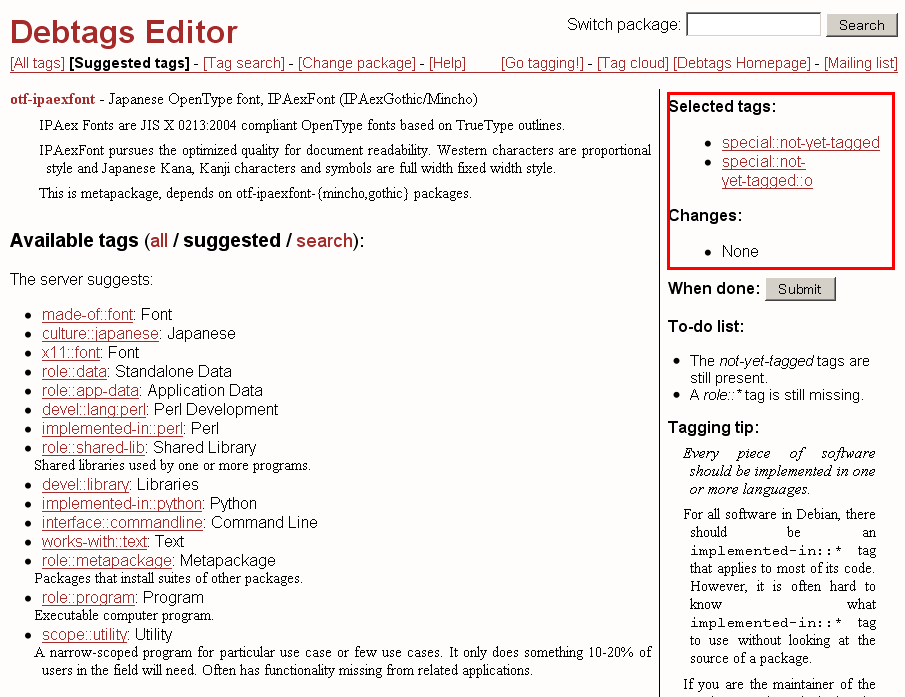
\includegraphics[height=0.5\hsize] {image201004/gotagging02.png}
 \caption{debtags タグ付け web インターフェイスの様子}
\label{fig:gotagging02}
\end{center}
\end{figure}

\begin{itemize}
 \item 選択したパッケージの説明(画面左上)
 \item 利用可能なタグの区別:all(すべて)/ suggested (おすすめ)/ search (検索)
 \item タグの一覧(画面左下)
 \item 既に付けられた・付けられるタグ(画面右)
\end{itemize}

\clearpage

\subsection{修正が必要なタグ}

まだキチンとタグ付けがされていないパッケージには、赤い×印と共に以下のような注意が表示されます。
ここからまず直していくことを考えましょう。

それぞれ以下のような意味合いです。

   \begin{table}[h]
    \begin{center}
      {
        \begin{tabular}{l|l} \hline
                表示される注意 & 意味合い \\ \hline \hline
The not-yet-tagged tags are still present. & このパッケージはまだタグ付けが終わってないよ、のタグが残ってます。 \\
An implemented-in::* tag seems to be missing. & このソフトはほげほげ言語で実装されています、ってタグ付けしようね \\
A role::* tag is still missing. & このソフトの役割をタグ付けせよ(role は必須です) \\
A devel::lang:* tag seems to be missing. & ほげほげ言語開発用のタグを付けましょう \\
           \end{tabular}
        }
     \caption{タグ付けがされていないパッケージの注意書き}
     \label{tagwarning}
    \end{center}
    \end{table}

これを踏まえて以下のような作業をします。

\begin{itemize}
 \item まだパッケージを指定していないなら、パッケージ名をクリック
 \item 提示されるタグや検索したタグをクリックして追加
 \item 必要ないタグが付けられている場合はクリックして削除
 \item 画面右側の「Selected tags:」と「Changes:」を見て、問題がないことを確認する
 \item 最後に submit 
\end{itemize}


\begin{figure}[H]
\begin{center}
 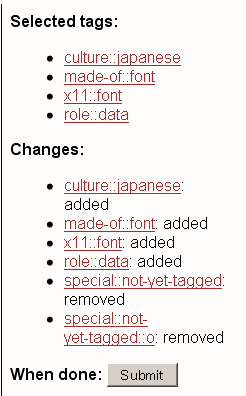
\includegraphics[height=0.5\hsize] {image201004/gotagging03.png}
 \caption{画面右側の「Selected tags:」と「Changes:」を確認!}
\label{fig:gotagging03}
\end{center}
\end{figure}


これだけで作業は終わりです。簡単ですね!


\subsection{どんなタグがあるの?}

タグ付け自体は簡単なものなので、パッケージに対して適切なタグを付けることが肝要なのですが、
すべてのタグを覚えることは大変すぎるのであきらめて、
サイトが適宜提示してくれるものの中から選択しましょう。
あと一応ガイドラインもあります (\url{http://wiki.debian.org/DebTaggingGuidelines})

で、最初に「推奨」タグが表示されています。適当なものがあればここから選ぶのもいいですが、お勧めは
\begin{itemize}
 \item 他の似たパッケージを見てみる→おんなじタグ使う
 \item all を選んで、検索窓からキーワードでタグを検索してみる
\end{itemize}
です。


\subsection{その他疑問点?}

\begin{itemize}
 \item 悪意のあるコミットについては? spammerなどは大丈夫?:

        コミットされたタグについては一応ブラウザのクッキーが紐付けられていて、レビュー時に重宝している模様です。

 \item コミットは誰でもできる?レビューは?:
 
        レビューするには Alioth の 'debtags' グループに参加する必要があるそうです。
        また少なくとも Debian を使っていないと、レビューの分類をする際、細かな点でうまく判断できないだろうということでした。
\end{itemize}


\subsection{最後に}
Happy tagging!

\printindex

\cleartooddpage

\vspace*{15cm}
\hrule
\vspace{2mm}

\includegraphics[width=2cm]{image200502/openlogo-nd.eps}
\noindent \Large \bf Debian 勉強会資料\\ \\
\noindent \normalfont \debmtgyear{}年\debmtgmonth{}月\debmtgdate{}日 \hspace{5mm}  初版第1刷発行\\
\noindent \normalfont 東京エリア Debian 勉強会 (編集・印刷・発行)\\
\hrule

\end{document}
